\section{La dinámica para la compuerta controlled-not}
El operador \textsc{CNOT} puede expandirse de la siguiente manera:
\begin{equation*}
        \cnot=\frac{1}{4}(\Id+\pauli{3}\otimes\Id+\Id\otimes\pauli{1}-\pauli{3}\otimes\pauli{1}).
\end{equation*}
Si se calcula el logaritmo de la compuerta es posible hallar el hamiltoniano generador de la unitaria,
\begin{equation*}
    H_{\cnot}=\frac{\pi}{4}\qty(\Id-\pauli{3}\otimes\Id-\Id\otimes\pauli{1}+\pauli{3}\otimes\pauli{1}),
\end{equation*}
que por ser una suma de operadores que conmutan entre sí, nos permite ver al controlled not como una aplicación consecutiva de tres unitarias diferentes
\begin{align*}
    \cnot&=e^{-i\frac{\pi}{4}\Id}e^{i\frac{\pi}{4}\pauli{3}\otimes\Id}e^{i\frac{\pi}{4}\Id\otimes\pauli{1}}e^{-i\frac{\pi}{4}\pauli{3}\otimes\pauli{1}}\\
    &=e^{-i\frac{\pi}{4}} (e^{i\frac{\pi}{4}\pauli{3}}\otimes \Id) (\Id \otimes e^{i\frac{\pi}{4}\pauli{1}}) e^{-i\frac{\pi}{4}\pauli{3}\otimes\pauli{1}}.
\end{align*}
De momento no le vi como sacarle jugo a esto, pero será útil para la extensión a tiempo arbitrario.
Escribiendo al estado de máxima entropía como $\varrho=\rho_{A}\otimes\rho_{B}$, la dinámica efectiva escribimos
\begin{equation*}
    \Gamma_{t}^{\mcM,\rho}[\rho(0)]=\frac{1}{2}[\rho(0)+p(\sigma_{3}\rho_{A}\sigma_{3}+\Tr{\sigma_{1}\rho_{B}}[\rho_{A}-\sigma_{3}\rho_{A}\sigma_{3}])+(1-p)(\sigma_{1}\rho_{B}\sigma_{1}+\Tr{\sigma_{3}\rho_{A}}[\rho_{B}-\sigma_{1}\rho_{B}\sigma_{1}])]
\end{equation*}
En términos del vector de Bloch, que es una forma rápida de obtener el cambio de los observables y de la esfera, la dinámica se ve como
\begin{equation*}
    \vec{r}_{\rho}=(pr_{A}+(1-p)r_{B})\hat{r}_{\rho}\mapsto\begin{pmatrix}
        r_{B}(pr_{A}(\hat{r}_{\rho,1})^2+(1-p)\hat{r}_{\rho,1})\\
        r_{B}r_{A}(p\hat{r}_{\rho,1}\hat{r}_{\rho,2}+(1-p)\hat{r}_{\rho,2}\hat{r}_{\rho,3})\\
        r_{A}(p\hat{r}_{\rho,3}+(1-p)r_{A}(\hat{r}_{\rho,3})^{2})
    \end{pmatrix}.
  \end{equation*}
  De momento tengo que ver esto en términos de matrices. El controlled not es una aplicación consecutiva de 3 unitarias, así que no debería ser demasiado complicado obtener la transformación de forma más elegante.


  \begin{figure}[h!]
    \centering
    \begin{subfigure}{0.45\textwidth}
      \centering
      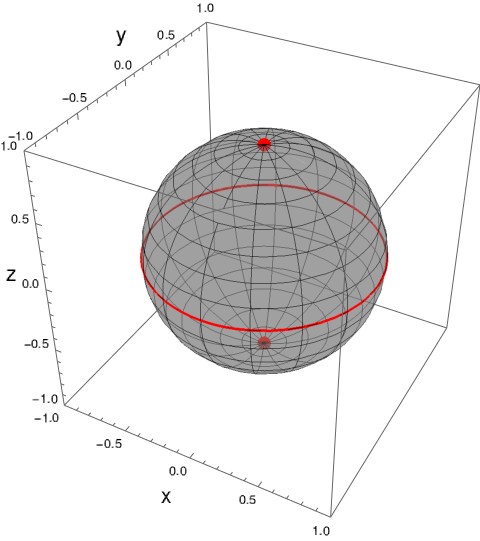
\includegraphics[width=0.9\linewidth]{maxent/figures/sphere_CNOT_t=0.0_z=0.8_p=0.95.png}
      \caption{$t=0$}
    \end{subfigure}%
    \begin{subfigure}{0.45\textwidth}
      \centering
      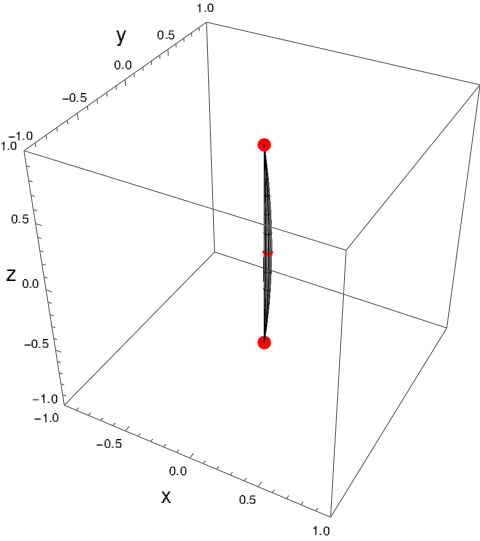
\includegraphics[width=0.9\linewidth]{maxent/figures/sphere_CNOT_t=1.0_z=0.8_p=0.95.png}
      \caption{$t=1.0$}
    \end{subfigure}
    \caption{Efecto de la evolución subyacente si $r=0.8$, $p=0.95$.}
    \label{fig:CNOTsequence2}
\end{figure}

\begin{figure}[h!]
    \centering
    \begin{subfigure}{0.45\textwidth}
      \centering
      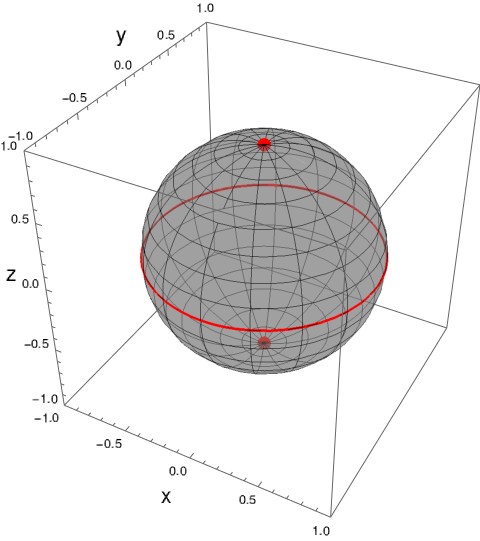
\includegraphics[width=0.9\linewidth]{maxent/figures/sphere_CNOT_t=0.0_z=0.8_p=0.6.png}
      \caption{$t=0$}
    \end{subfigure}%
    \begin{subfigure}{0.45\textwidth}
      \centering
      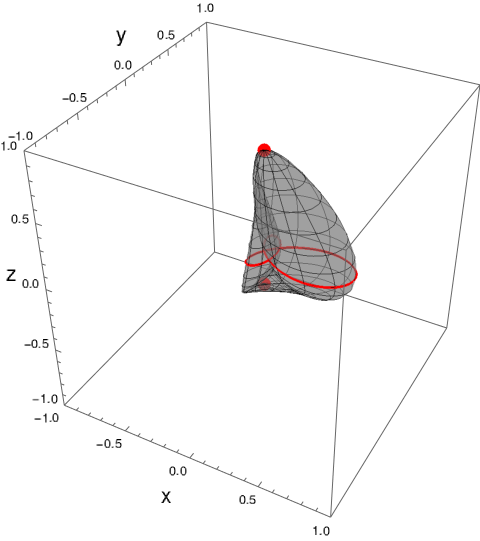
\includegraphics[width=0.9\linewidth]{maxent/figures/sphere_CNOT_t=1.0_z=0.8_p=0.6.png}
      \caption{$t=1.0$}
    \end{subfigure}
    \caption{Efecto de la evolución subyacente si $r=0.8$, $p=0.6$.}
    \label{fig:CNOTsequence2}
\end{figure}